%%% %%%%%%%%%%%%%%%%%%%%%%%%%%%% %%%
%%% Main Chapter 2 : Challenges  %%%
%%% %%%%%%%%%%%%%%%%%%%%%%%%%%%% %%%
\chapter{Experimente}
\label{chap:experiments}

In diesem Kapitel werden die einzelnen Experimente beschrieben, mit denen einige Neuerungen und auch Probleme der jeweiligen Version getestet werden können. Es soll später als Experimentierhandbuch verwendet werden können.

Jeder Abschnitt beschreibt zunächst die notwendigen Vorbereitungen.
Anschließgend folgt eine Serie von Handlungsanweisungen.
Schließlich folgt eine Erklärung des erwarteten Verhalten und Möglichkeiten diese zu Beobachten.


%Was tun?
%Was beobachten?
%Aufbau?
%erwartetes Verhalten?

%Bspw. Übung: TSR durch Memory Abbild

%%%%%%%%%%%%%%%%%%%%%%%%%%%%%%%%%%%%%%%%%%%%%%%%%%%%%%%%%%%%%%%%%%%%%%%%%%%%%%%%%%%%%%%%%%%%%%%%%%%%%%%%%
\section{DOS 5.0}
%%%%%%%%%%%%%%%%%%%%%%%%%%%%%%%%%%%%%%%%%%%%%%%%%%%%%%%%%%%%%%%%%%%%%%%%%%%%%%%%%%%%%%%%%%%%%%%%%%%%%%%%%


	\subsection{TSR}

	Unter MS DOS konnten noch keine Anwendungen parallel ausgeführt werden. Insbesondere waren  Daemons oder Backgroundprozesse nicht vorgesehen.
	Um zu kleinen Tools wie bspw. einem Taschenrechner wechseln zu können, ohne die eigentliche Anwendung beenden zu müssen, konnte man sich mit sogenannten TSRs, "`Teminate and Stay Resident"'-Programmen behelfen\footnote{Eine hervorragende Einführung in die Programmierung und die Funktionsweise von TSRs befindet sich unter: \url{https://courses.engr.illinois.edu/ece390/books/artofasm/CH18/CH18-1.html\#HEADING1-3}}.
	%Ebenso waren die meisten Computerviren zu dieser Zeit TSRs. 

	\begin{figure}[h]
		\begin{center}
			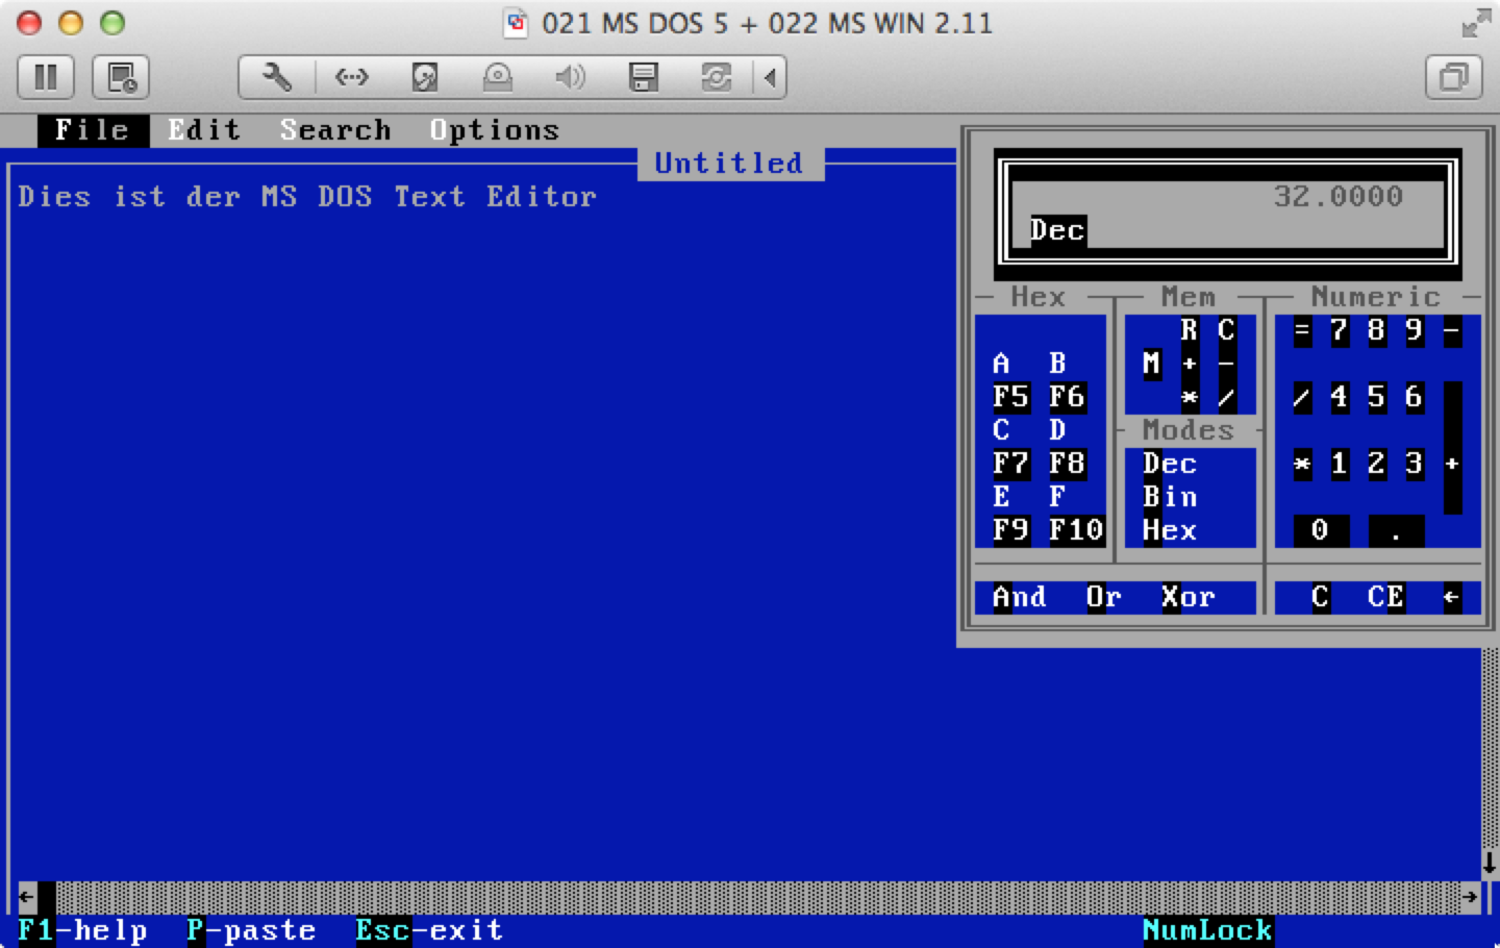
\includegraphics[width=0.8\textwidth]{img/dostsr}
			\caption{TSR-Taschenrechner vor dem DOS-Editor}
			\label{fig:screenshot-dostsr}
		\end{center}
	\end{figure}

	Eine sehr beliebte TSR war Borland Sidekick, die unter anderm einen Notizzettel, einen Taschenrechner und einen Kalender bereitstellte. Mit dem Befehl ctrl+alt konnte man diese jederzeit aufrufen.

	Machen Sie sich nun mit der Funktionsweise dieser TSR vertraut:
	
		\begin{itemize}
			\item Starten Sie die VM und beenden Sie die DOS Shell. Notieren Sie zunächst den freien Speicher, der mit dem Befehl \texttt{mem} ausgegeben werden kann.
			\item Starten Sie Sidekick (\texttt{$C:\backslash{}sk\backslash{}sk.com$}). Dieses Programm beendet sich sofort wieder. Überprüfen Sie erneut den freien Speicher. Wodurch kommt die Veränderung zustande?
			\item Starten Sie ein anderes Programm, zum Beispiel den Standard DOS Texteditor \texttt{EDIT}. Testen Sie dabei die Verwendung der Funktionen von Sidekick. Wodurch gelingt es Sidekick, wieder in den Vordergrund zu treten, obwohl die CPU an eine andere Anwendung abgegeben wurde?
			\item Was passiert bei der Verwendung einer TSR unter Windows?
		\end{itemize}
	  

	\subsection{Busy Waiting}

	Obwohl seit dem 8088er vorhanden, benutzt MS DOS noch nicht die \texttt{HLT}-Instruction der x86 CPU.
	
	\begin{itemize}
		\item Starten Sie die MS DOS VM und beobachten Sie ihr Verhalten. Beenden Sie hierzu die DOS Shell
		\item Wie viel CPU und wie viel RAM verbraucht die VM? Wie verändern sich diese Parameter unter Last? Wie verhält sich MS DOS folglich im Leerlauf?
		\item Starten Sie nun die Anwendung \texttt{DOSIDLE}. Um was für eine Anwendung handelt es sich?
		\item Wie hat sich die Ressourcennutzung der VM durch den Start der Anwendung verändert? Wodurch könnte dies erreicht werden?
	\end{itemize}


	\subsection{DOS-Shell}

	MS DOS wird in Version 5 wird mit einer an den Norton Commander angelehnten graphischen Shell ausgeliefert. Diese wird beim Start des Betriebssystems automatisch geladen.

	\begin{itemize}
		\item Machen Sie sich mit der Bedienung der DOS Shell vertraut. Benutzen Sie hierfür die $Alt$-Taste, um in die Menüs zu gelangen.
		\item Wie können aus dieser Shell Anwendungen gestartet werden? Starten und beenden Sie den Basic Interpreter QBasic
		\item Was passiert, wenn eine TSR, z.B. Sidekick aus der DOS Shell gestartet wird? 
	\end{itemize}

%%%%%%%%%%%%%%%%%%%%%%%%%%%%%%%%%%%%%%%%%%%%%%%%%%%%%%%%%%%%%%%%%%%%%%%%%%%%%%%%%%%%%%%%%%%%%%%%%%%%%%%%%
\section{Windows 2.11}
%%%%%%%%%%%%%%%%%%%%%%%%%%%%%%%%%%%%%%%%%%%%%%%%%%%%%%%%%%%%%%%%%%%%%%%%%%%%%%%%%%%%%%%%%%%%%%%%%%%%%%%%%

	\subsection{Koop. Multitasking}

	Anders als unter MS DOS können unter Windows mehrere Anwendungen gleichzeitig ausgeführt werden. 
	Dadurch ist die Verwendung von TSRs nicht mehr notwendig.

	\begin{itemize}
		\item Starten Sie Microsoft Windows 2.11 und machen Sie sich mit den mitgelieferten Applikationen vertraut.
		\item Starten Sie Microsoft Excel und eine weitere Anwendung. Wie ist Copy \& Paste implementiert?
		\item Was passiert beim Absturz einer Anwendung? Warum?
	\end{itemize}


%%%%%%%%%%%%%%%%%%%%%%%%%%%%%%%%%%%%%%%%%%%%%%%%%%%%%%%%%%%%%%%%%%%%%%%%%%%%%%%%%%%%%%%%%%%%%%%%%%%%%%%%%
\section{DOS 6.22}
%%%%%%%%%%%%%%%%%%%%%%%%%%%%%%%%%%%%%%%%%%%%%%%%%%%%%%%%%%%%%%%%%%%%%%%%%%%%%%%%%%%%%%%%%%%%%%%%%%%%%%%%%

	\subsection{Extended Memory}

	MS DOS verwendet den Real Mode der x86 CPU, indem diese aufgrund der Registerbreite maximal 1 MiB RAM adressieren kann. Davon stellt MS DOS bis zu 640kiB Anwendungen zur Verfügung. Ende der 80er war dies jedoch für die meisten Programme bereits deutlich zu wenig.

	\begin{itemize}
		\item Starten Sie Microsoft Windows 2.11 und machen Sie sich mit den mitgelieferten Applikationen vertraut.
		\item Starten Sie Microsoft Excel und eine weitere Anwendung. Wie ist Copy \& Paste implementiert?
		\item Was passiert beim Absturz einer Anwendung? Warum?
	\end{itemize}

	\subsection{DoubleSpace oder DriveSpace}

	Ein häufiges Problem zur Zeit von MS DOS war der begrenze Speicherplatz. Mit MS DOS 6.0 wurde daher die Datenträgerkomprimierung DoubleSpace eingeführt.
	Diese musste aus patentrechtlichen Gründen jedoch von Microsoft bald wieder entfernt werden und wurde mit DOS 6.22 durch DriveSpace, ein Programm mit ähnlicher Funktionsweise aber anderem Kompressionsalgorithmus ersetzt.

	\begin{itemize}
		\item Starten Sie die VM und legen Sie das mitgelieferte, leere 1,44MB-Diskettenimage in Laufwerk A: ein.
		\item Erzeugen Sie mit dem Befehl Type eine Textdatei mit einer Größe von mindestens 1,5 MB.
		Was passiert, wenn Sie versuchen, diese auf Volume A: zu kopieren?
		\item Legen Sie mittels DriveSpace ein komprimiertes Dateisystem auf diesem Image an. Lesen Sie hierfür ggf. $help drvspace$.
		\item Versuchen Sie erneut, die Textdatei auf Volume A: zu kopieren. 
		\item Wie unterscheiden sich die Werte des $Volume$ und der $dir$-Kommandos?
	\end{itemize}

%%%%%%%%%%%%%%%%%%%%%%%%%%%%%%%%%%%%%%%%%%%%%%%%%%%%%%%%%%%%%%%%%%%%%%%%%%%%%%%%%%%%%%%%%%%%%%%%%%%%%%%%%
\section{Windows 3.11 for Workgroups}
%%%%%%%%%%%%%%%%%%%%%%%%%%%%%%%%%%%%%%%%%%%%%%%%%%%%%%%%%%%%%%%%%%%%%%%%%%%%%%%%%%%%%%%%%%%%%%%%%%%%%%%%%

	\subsection{Netzwerk}

		Windows 3.11 ermöglicht erstmals Datei- und Printersharing über das SMB-Protokoll.
	
		\begin{itemize}
			\item Legen Sie zunächst eine Heimnetzgruppe auf mindestens zwei virtuellen Maschinen an.
			\item Kopieren Sie eine Datei von ihrem Übungspartner.
		\end{itemize}

	\subsection{Internetzugriff}

		Ebenfalls ab Windows 3.11 ist der Zugriff auf das Internet möglich.
		Hierfür wurde das TCP/IP-Protokoll nachgerüstet. 

		\begin{itemize}
			\item Starten Sie den vorinstallierten Internet Explorer 5.
			\item Rufen Sie nun einige Webseiten auf und vergleichen Sie, wie sehr sich das Internet in den letzten 20 Jahren gewandelt hat. Können Sie ein aktuelle Webseite finden, die fehlerfrei dargestellt wird?
			\item Ebenfalls installiert ist der Netscape Navigator 4.
		Dieser ist auf neuen CPUs durch einen Bug nicht lauffähig und stürzt beim Start ab. 
		Warum stürzt hierbei das gesamte Betriebssystem ab?
		\end{itemize}

%%%%%%%%%%%%%%%%%%%%%%%%%%%%%%%%%%%%%%%%%%%%%%%%%%%%%%%%%%%%%%%%%%%%%%%%%%%%%%%%%%%%%%%%%%%%%%%%%%%%%%%%%
\section{Windows NT 3.51}
%%%%%%%%%%%%%%%%%%%%%%%%%%%%%%%%%%%%%%%%%%%%%%%%%%%%%%%%%%%%%%%%%%%%%%%%%%%%%%%%%%%%%%%%%%%%%%%%%%%%%%%%%

	\subsection{NTFS}
	Streams, Hidden files
	lange vs. kurze Dateinamen
	mehrere Namen pro File

	\subsection{VGA im User Mode}

%%%%%%%%%%%%%%%%%%%%%%%%%%%%%%%%%%%%%%%%%%%%%%%%%%%%%%%%%%%%%%%%%%%%%%%%%%%%%%%%%%%%%%%%%%%%%%%%%%%%%%%%%
\section{Windows NT 4.0 SP 6}
%%%%%%%%%%%%%%%%%%%%%%%%%%%%%%%%%%%%%%%%%%%%%%%%%%%%%%%%%%%%%%%%%%%%%%%%%%%%%%%%%%%%%%%%%%%%%%%%%%%%%%%%%

	\subsection{CSRSS}
	\subsection{EXEType}

%%%%%%%%%%%%%%%%%%%%%%%%%%%%%%%%%%%%%%%%%%%%%%%%%%%%%%%%%%%%%%%%%%%%%%%%%%%%%%%%%%%%%%%%%%%%%%%%%%%%%%%%%
\section{Windows 2000 Professional}
%%%%%%%%%%%%%%%%%%%%%%%%%%%%%%%%%%%%%%%%%%%%%%%%%%%%%%%%%%%%%%%%%%%%%%%%%%%%%%%%%%%%%%%%%%%%%%%%%%%%%%%%%

	\subsection{Active Directory}
	\subsection{EFS?}

